\documentclass[tikz,border=9pt]{standalone}
\usepackage{amsmath,amssymb}
\usetikzlibrary{arrows.meta,positioning,calc}
\begin{document}
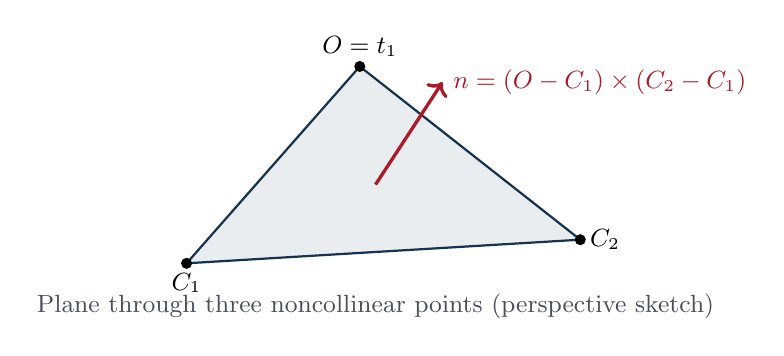
\begin{tikzpicture}[font=\small,arr/.style={-{Stealth},thick},box/.style={draw=blue!55!black,rounded corners,fill=blue!4,align=center,text width=2.9cm,minimum height=1.05cm}]
\definecolor{navy}{RGB}{21,50,78}\definecolor{solveRed}{RGB}{171,26,40}\definecolor{muted}{RGB}{70,79,92}

\coordinate (A) at (0,0); \coordinate (B) at (5,.3); \coordinate (C) at (2.2,2.5);
\fill[navy!9] (A)--(B)--(C)--cycle;
\draw[navy,thick] (A)--(B)--(C)--cycle;
\fill (A) circle(2pt) node[below]{$C_1$}; \fill (B) circle(2pt) node[right]{$C_2$};
\fill (C) circle(2pt) node[above]{$O=t_1$};
\draw[solveRed,very thick,->] (2.4,1)--(3.25,2.3) node[right]{$n=(O-C_1)\times(C_2-C_1)$};
\node[muted] at (2.4,-.55){Plane through three noncollinear points (perspective sketch)};

\end{tikzpicture}
\end{document}
